\documentclass[twoside]{article}

\usepackage{diagbox}
\usepackage{mathtools}

\usepackage{amsmath,amsthm}
\usepackage{xspace}
\usepackage{fancyhdr}
\usepackage{hyperref}
\usepackage[a4paper,left=2cm,right=2cm,top=2cm,bottom=2cm]{geometry}
\newtheorem{definition}{Definition}
%%% Logik


% !TEX root =  main.tex

\newcommand{\DiMo}{\textsc{DiMo}\xspace}

\newcommand{\Var}{\ensuremath{\mathcal{V}}}
\newcommand{\AL}{\textup{AL}}
\newcommand{\FO}{\textup{FO}}
\newcommand{\logtrue}{\ensuremath{\mathtt{t\!t}}}
\newcommand{\logfalse}{\ensuremath{\mathtt{f\!f}}}
\newcommand{\imp}{\ensuremath{\rightarrow}}
\newcommand{\biimp}{\ensuremath{\leftrightarrow}}
\newcommand{\length}[1]{\ensuremath{\mathit{len}(#1)}}
\newcommand{\size}[1]{\ensuremath{|#1|}}
\newcommand{\arity}[1]{\ensuremath{\mathit{arity}(#1)}}
\newcommand{\free}[1]{\ensuremath{\mathit{free}(#1)}}
\newcommand{\bound}[1]{\ensuremath{\mathit{bnd}(#1)}}
\newcommand{\weight}[1]{\ensuremath{|\!|#1|\!|}}
\newcommand{\sub}[1]{\ensuremath{\mathit{Sub}(#1)}}
\newcommand{\Mod}[1]{\ensuremath{\mathit{Mod}(#1)}}
\newcommand{\Th}[1]{\ensuremath{\mathit{Th}(#1)}}
\newcommand{\satequiv}{\ensuremath{\equiv_{\mathsf{sat}}}}
\newcommand{\yields}{\ensuremath{\Longrightarrow}}
\newcommand{\sem}[3]{\ensuremath{[\![ #1 ]\!]_{#2}^{#3}}}

\renewcommand{\phi}{\varphi}

\newcommand{\term}[1]{\ensuremath{\texttt{#1}\ }}
\newcommand{\nonterm}[1]{\ensuremath{\langle\mathit{#1}\rangle\ }}
\newcommand{\optional}[1]{\ensuremath{\Big[\ #1\ \Big]}}
\newcommand{\enumset}[1]{\ensuremath{\Big\{#1\Big\}}}
\newcommand{\group}[1]{\ensuremath{\Big(#1\Big)}}
\newcommand{\altn}{\ensuremath{\enspace\rule[-2mm]{.4pt}{6mm}}\enspace}

%%%%%%%%%%%%%%% TODO comments %%%%%%%%%%%
\newcounter{TODOcounter}
\newcommand{\TODO}[1]{%
	\stepcounter{TODOcounter}%
	{{\color{red}\scriptsize\bf$^{(\arabic{TODOcounter})}$}}%
	\marginpar[\fbox{%
		\parbox{3cm}{\scriptsize{\color{red}\raggedleft%
				$^{({\bf{\arabic{TODOcounter}}})}$%
				#1}}}]%
	{\fbox{\parbox{3cm}{\scriptsize{\color{red}\raggedright% 
					$^{({\bf{\arabic{TODOcounter}}})}$%
					#1}}}}%
}


\newcommand{\DiMoVersion}{0.3.0}


\title{\DiMo -- A Tool for Discrete Modelling Using Propositional Logic \\ Version \DiMoVersion}

\author{Martin Lange, Maurice Herwig \\ University of Kassel, Germany}


\fancyhead[L]{M.~Lange, M.~Herwig}
\fancyhead[R]{The \DiMo Tool}
\fancyfoot[RO, LE]{\thepage}
\fancyfoot[C]{}
\renewcommand{\headrulewidth}{0.4pt}
\renewcommand{\footrulewidth}{0.4pt}
\pagestyle{fancy}


\allowdisplaybreaks

\begin{document}

\maketitle

\tableofcontents

\section{Discrete Modelling Problems}

The \DiMo language can be used to model various discrete decision or computation problems as logical problems in quantifier-free logic.
The four logical problems that are supported are
\begin{itemize}
\item the \emph{satisfiability problem} for finding \emph{some} model of a given formula;
\item the \emph{validity problem} for checking whether \emph{all} interpretations satisfy a given formula, respectively for finding
      a countermodel;
\item the \emph{model class} problem for finding \emph{all} models of a given formula;
\item the \emph{equivalence} problem for checking whether two given formulas are semantically equivalent on a given set of propositions, 
      respectively finding a model (in those propositions) that separates the two.
\end{itemize}
The \DiMo language can be used to specify formulas \emph{parametrised} by natural numbers. The logical problems above are then applied
to \emph{all} instances of such formula schemes. 


\section{Basic Design Principles of the Language}

\paragraph*{Specifying problems.} 
A \DiMo input starts with the specification of the problem, defined by the keywords \texttt{SATISFIABLE}, \texttt{VALID}, 
\texttt{EQUIVALENT} or \texttt{MODELS}, followed by the formula scheme to be tested and the output control. 

In case of the equivalence problem this is followed by the keyword \texttt{TO} and a second formula scheme. Note that this is a generalisation
of the standard equivalence problem which checks equality between the model classes of two formulas. Here the input is given by two formulas
$\varphi$ and $\psi$ and a set of propositional variables $L$, and the question is to decide whether the model classes of $\varphi$ and $\psi$
coincide when restricted to $L$. In other words: for every propositional variable assignment $\vartheta$ s.t.\ $\vartheta \models \varphi$, is
there a variable assignment $\vartheta'$ s.t.\ $\vartheta' \models \psi$ and $\vartheta(X) = \vartheta'(X)$ for all $X \in L$. Moreover, does
the same hold vice-versa between $\psi$ and $\varphi$? Note that this generalises semantic equivalence in the sense that each pair of
semantically equivalent formulas is also equivalent when restricted to any $L$ but not vice-versa.
 

\paragraph*{Specifying interesting predicates.}
One can then optionally specify the (names) of the predicate symbols which should be considered in the output. This can be used to interact with these predicates in the control of the output program flow. 
This is indicated by the keyword \texttt{PROPOSITIONS}, followed by a list of those predicate names. Note
that all predicate symbols not listed here can't use in the output controll. Hence, without the \texttt{PROPOSITIONS} section in the input, no models / 
countermodels are generated.

Furthermore, when the chosen problem is the equivalence problem then it is taken to be restricted to those propositions that are given 
in this section. Consequently, when no propositions are given here, the equivalence problem boils down to a simple equi-satisfiability check.

\paragraph*{Specifying parameters.}
This section is followed by a section specifying the parameters to the formula scheme, started with the keyword \texttt{PARAMETERS}.
Parameters are variables for natural numbers and can be denoted with an arbitrary alphanumeric string starting with a lowercase letter.
Parameters to the scheme are specified as a comma-separated list of name-domain pairs, for instance 
\begin{quote}
\texttt{n : NAT}   
\end{quote}
defines a parameter \texttt{n} that stands for any number in $\{0,1,\ldots\}$. Other means to specify a domain are, for instance
\begin{center}
\begin{tabular}{ll}
\texttt{\{3,..\}} & for the set $\{3,4,5,\ldots\}$, \\
\texttt{\{3,7,..\}} & for the set $\{3,7,11,15,\ldots\}$, \\
\texttt{\{3,7,..,20\}} & for the set $\{3,7,11,15,19\}$, \\
\texttt{\{3,7,20,4,16\}} & for the set $\{3,4,7,16,20\}$.
\end{tabular}
\end{center} 
It is possible to impose certain simple conditions on parameter combinations by appending the keyword \texttt{WITH}, followed by
a comma-separated non-empty list of basic comparisons like \texttt{n < m}. Allowed comparisons are \emph{equals}, \emph{greater-than}, 
\emph{less-than}, \emph{greater-or-equals}, \emph{less-or-equals}, and \emph{unequals}.

\paragraph*{Specifying formula abbreviations.} 
There is no distinction between a predicate, like \texttt{P(n,m)} and an auxiliary formula. It is thus possible to abbreviate certain
formula parts and give the definition of these predicates in a final section started with the keyword \texttt{WHERE}, followed by
a list of definitions of the form 
\begin{quote}
\emph{pattern} \texttt{=} \emph{formula}
\end{quote}
Note that there is no comma separation between these definitions. A pattern in this context is a predicate symbol, possibly followed
by a comma-separated list of variables or numbers, enclosed in parentheses, i.e.\ \texttt{P} or \texttt{P(n)} or \texttt{P(0,n)}.
Note that \DiMo does not type-check predicates w.r.t.\ their arity. A symbol should only be used with the same arity throughout the
entire specification.

\paragraph*{Specifying terms and finite sets.} 
Terms are made up from integers and variables which are either specified in the \texttt{PARAMETERS} section or introduced by the junctors 
\texttt{FORALL} and \texttt{FORSOME}, using the arithmetical operations of addition, subtraction and multiplication. Terms can be used
as arguments to predicate symbols, for instance as in \texttt{X(n,n+2)}.

A finite set is an enumeration of terms like \texttt{\{1,n,n+3,m-2,n*m+i,10\}}. It is possible to define linear sets by specifying the
least, possibly the second-to-least, and the last element. This follows the same convention as used in the specification of domains
above. For instance, \texttt{\{1,..,n\}}, \texttt{\{0,2,..,n-1\}} and \texttt{\{n,2*n,..,m*n\}} are valid specifications of such sets
provided that the variables have been defined either as parameters or via generalised junctors, see below.

There are also the operators \texttt{MIN} and \texttt{MAX} which turn sets into terms. For instance, \texttt{MIN \{n+1,9,k,m-n\}} is a term.


\paragraph*{Specifying formulas.}
The \DiMo language supports propositional logic with the standard Boolean unary or binary operators $\wedge,\vee,\neg,\to,\leftrightarrow$, 
as well as conjunctions and disjunctions over finite sets of indices (e.g.\ $\bigwedge_{i=1}^n \ldots$). For instance, formula (scheme)
$\bigwedge_{i=0}^{n-1} X_i \leftrightarrow X_{i+1}$, parametrised by a natural number $n$ would be specified as
\begin{quote} \tt
  FORALL i: \{0,..,n-1\} . X(i) <-> X(i+1)
\end{quote}
In general, such a junctor defines a new variable \texttt{i} which can be used in the formula following the dot. A disjunction $\bigvee$ 
is denoted using the keyword \texttt{FORSOME}.


 


\section{Examples}

\subsection{The $n$-Queens Problem}\label{n-queens}

A standard discrete modelling problem is the following: given a chess board of size $n \times n$ with $n \ge 1$, place $n$ queens on this board such that
none of them threatens another. A queen in chess can move an arbitrary distance along a row, column or diagonale. Clearly, the problem
amounts to placing one queen in each column for example. Moreover, to exclude possible threats between queens, by symmetry it suffices to
consider one direction per row/column/diagonale only, for example no queen should ``see'' another queen in the directions east, north, 
north-east and south-east. 

The question of finding a solution to the $n$-queens problem boils down to finding a model of the following propositional formula (scheme) $\varphi_n$ for
given $n$. We use propositional variables $D_{i,j}$ with $1 \le i,j, \le n$ to intuitively denote that the square in column $i$ and row $j$ is occupied by a queen.
\begin{align*}
\varphi_n := & \bigwedge\limits_{i=1}^n \bigvee\limits_{j=1}^n D_{i,j} & \text{``\emph{in each column place a queen in some row}''} \\
\wedge & \bigwedge\limits_{i=1}^n \bigwedge\limits_{j=1}^{n-1} D_{i,j} \to \bigwedge\limits_{k=j+1}^n \neg D_{i,k} & \text{``\emph{no two queens per row}''} \\ 
\wedge & \bigwedge\limits_{i=1}^{n-1} \bigwedge\limits_{j=1}^n D_{i,j} \to \bigwedge\limits_{k=i+1}^n \neg D_{k,j} & \text{``\emph{no two queens per column}''} \\ 
\wedge & \bigwedge\limits_{i=1}^{n-1} \bigwedge\limits_{j=1}^{n-1} D_{i,j} \to \hspace*{-1cm} 
  \bigwedge\limits_{k = 1 \atop \text{s.t. } i+k \le n \text{ and } j+k \le n}^\infty \hspace*{-1cm}\neg D_{i+k,j+k} 
  & \text{``\emph{no two queens per diagonale up}''} \\ 
\wedge & \bigwedge\limits_{i=1}^{n-1} \bigwedge\limits_{j=2}^{n} D_{i,j} \to \hspace*{-1cm} 
  \bigwedge\limits_{k = 1 \atop \text{s.t. } i+k \le n \text{ and } j-k \ge 1}^\infty \hspace*{-1cm}\neg D_{i+k,j-k} 
  & \text{``\emph{no two queens per diagonale down}''} \\ 
\end{align*}
The problem of finding a model for each instance of $\varphi_n$ can be specified as a \DiMo program as follows.
\begin{verbatim}
SATISFIABLE NQueens(n)
PROPOSITIONS D
PARAMETERS n: {1,..}
FORMULAS 
  NQueens(n) = AtLeastOneInEachRow(n)
             & AtMostOneInEachRow(n)
             & AtMostOneInEachColumn(n)
             & AtMostOneInEachDiagUp(n)
             & AtMostOneInEachDiagDown(n)
	         
  AtLeastOneInEachRow(n)     = 
    FORALL i: {1,..,n}. FORSOME j: {1,..,n}. D(i,j)
    
  AtMostOneInEachRow(n)      = 
    FORALL i: {1,..,n}. FORALL j: {1,..,n-1}. 
      D(i,j) -> FORALL k: {j+1,..,n}. -D(i,k)
    
  AtMostOneInEachColumn(n)   = 
    FORALL i: {1,..,n-1}. FORALL j: {1,..,n}. 
      D(i,j) -> FORALL k: {i+1,..,n}. -D(k,j)
    
  AtMostOneInEachDiagUp(n)   = 
    FORALL i: {1,..,n-1}. FORALL j: {1,..,n-1}. 
      D(i,j) -> FORALL k: {1,..,MIN {n-i,n-j}}. -D(i+k,j+k)
    
  AtMostOneInEachDiagDown(n) = 
    FORALL i: {1,..,n-1}. FORALL j: {2,..,n}. 
      D(i,j) -> FORALL k: {1,..,MIN {n-i,j-1}}. -D(i+k,j-k)
\end{verbatim}
Testing this problem with the \DiMo tool reveals solutions in terms of propositional variable assignments from which the placement of queens on the 
chess boards of respective sizes can immediately be derived.
\begin{verbatim}
[~] dimo.native examples/nQueens.dm
Instance n=1 ................................... satisfiable.
  Satisfying assignment: D(1,1)
Instance n=2 ................................... unsatisfiable.
Instance n=3 ................................... unsatisfiable.
Instance n=4 ................................... satisfiable.
  Satisfying assignment: -D(1,1), -D(1,2), D(1,3), -D(1,4), D(2,1), -D(2,2), -D(2,3), 
  -D(2,4), -D(3,1), -D(3,2), -D(3,3), D(3,4), -D(4,1), D(4,2), -D(4,3), -D(4,4)
...
\end{verbatim} 
The output shows that the \DiMo tool has chosen the standard enumeration $n = 1,2,\ldots$ for the parameter \texttt{n}, instantiated the formulas scheme for
each instance of this enumeration and checked each of them for satisfiability subsequently. For $n = 2$ and $n = 3$ there is no solution to the $n$-queens
problem as one can easily check. Consequently, these instances are reported as being unsatisfiable. On the other hand, the instances $n=1,4,5,\ldots$ are
satisfiable, and a propositional model is found. It is easy to read off a solution to the $n$-queens problem from the assignment satisfying the $n$-th formula,
given the interpretation of the propositions $D_{i,j}$ mentioned above.

 
\subsection{A Simple Combinatorial Problem}

As a second example we consider the simple combinatorial problem of choosing exactly $m$ out of $n$ items. This can equally be modelled as the problem
of finding some or all models of a propositional formula $\varphi_{n,m}$ with $n \ge 1$ and $0 \le m \le n$. We use propositions $A_i$ to denote that
the $i$-th element is chosen. The straight-forward scheme
\begin{displaymath}
\bigvee\limits_{I \subseteq \{1,\ldots,n\} \atop |C| = m} (\bigwedge\limits_{i \in I} A_i) \wedge \hspace*{-5mm} \bigwedge\limits_{i \in \{1,\ldots,n\} \setminus I} \hspace*{-5mm} \neg A_i) 
\end{displaymath}
cannot be written down as such in the \DiMo language because variables for sets of natural numbers are not supported (yet). However, note that this 
is a formula of size $\mathcal{O}(n \cdot \binom{n}{m}) = \mathcal{O}(n^{m+1})$, and there is a much shorter way of specifying this which uses formulas
of size $\mathcal{O}(n^2)$ only. The trick is to use auxiliary propositions $B_{i,j}$ to abbreviate the fact that at least $j$ out of the first $i$
elements have chosen, or equivalently, at least $j$ of the $A_1,\ldots,A_i$ need to be set to true. Consider
\begin{align*}
\varphi_{n,m} := &B_{n,m}  & \text{``\emph{at least m out of (the first) n are chosen''}} \\ 
\wedge &\bigwedge\limits_{i=1}^n \bigwedge\limits_{j=1}^m B_{i,j} \to & \text{``\emph{if j of i are chosen then}} \\
&\hspace*{2.4cm} A_i \wedge B_{i-1,j-1} & \text{\emph{the i-th is chosen and j-1 of i-1 are chosen}} \\
&\hspace*{2cm}\vee B_{i-1,j} &\text{\emph{or j of i-1 are chosen}''} \\
\wedge &\bigwedge\limits_{j=1}^m \neg B_{0,j} & \text{``\emph{it is impossible to choose j from 0 elements}''}
\end{align*}
Using the same principle one can also demand that at the same time \emph{at most} $m$ out of $n$ are chosen. Note that this is the case if and only if
\emph{at least} $n-m$ are \emph{not chosen}. Based on this, the following \DiMo program specifies the problem of choosing exactly $m$ out $n$ elements
represented by propositions $A_i$. The auxiliary propositions $B_{i,j}$ are hidden away from output by not listing them in the \texttt{PROPOSITIONS}
section.
\begin{verbatim}
MODELS       ExactlyMofN(n,m)
PROPOSITIONS A
PARAMETERS   n : {1,..}, m : NAT WITH m <= n
FORMULAS

  ExactlyMofN(n,m) = AtLeastMChosen(n,m) & AtMostMChosen(n,m)

  AtLeastMChosen(n,m) = B(n,m) & BsWellBehaved(n,m) & BsEndOk(m)
  BsWellBehaved(n,m)  = FORALL i : {1,..,n}. FORALL j: {1,..,m}. 
                          B(i,j) -> A(i) & B(i-1,j-1) | B(i-1,j) 
  BsEndOk(m)          = FORALL j : {1,..,m}. -B(0,j)

  AtMostMChosen(n,m) = AtLeastNminusMNotChosen(n,n-m)
  AtLeastNminusMNotChosen(n,m) = N(n,m) & NsWellBehaved(n,m) & NsEndOk(m)
  NsWellBehaved(n,m) = FORALL i : {1,..,n}. FORALL j: {1,..,m}. 
                          N(i,j) -> -A(i) & N(i-1,j-1) | N(i-1,j)
  NsEndOk(m)         = FORALL j : {1,..,m}. -N(0,j)
\end{verbatim}
Note that formulas constraining the propositions \texttt{N(i,j)} are copied verbatim from those for the \texttt{B(i,j)}. It is not (yet) possible to
re-use such code because only integer variables can be used as parameters, not propositions themselves. 

Running the \DiMo tool on this program results in finding all possibilities to choose $m$ out of $n$ elements, represented by propositional variable
assignments, for some enumeration of the parameters $n$ and $m$.
\begin{verbatim}
[~] dimo.native examples/exactlyMofN.dm
Instance m=0, n=1 .............................. 
  Found model -A(1)
1 model found.
Instance m=0, n=2 .............................. 
  Found model -A(1), -A(2)
1 model found.
Instance m=1, n=1 .............................. 
  Found model A(1)
1 model found.
Instance m=0, n=3 .............................. 
  Found model -A(1), -A(2), -A(3)
1 model found.
Instance m=1, n=2 .............................. 
  Found model A(1), -A(2)
  Found model -A(1), A(2)
2 models found.
Instance m=0, n=4 .............................. 
  Found model -A(1), -A(2), -A(3), -A(4)
1 model found.
Instance m=1, n=3 .............................. 
  Found model A(1), -A(2), -A(3)
  Found model -A(1), A(2), -A(3)
  Found model -A(1), -A(2), A(3)
3 models found.
Instance m=2, n=2 .............................. 
  Found model A(1), A(2)
1 model found.
Instance m=0, n=5 .............................. 
  Found model -A(1), -A(2), -A(3), -A(4), -A(5)
1 model found.
...
\end{verbatim}
The chosen enumeration of all pairs of parameters $n,m$ such that $n \ge 1$, and $0 \le m \le n$ is the standard ``diagonale'' $(1,0),(2,0),(1,1),(3,0),(2,1),(4,0),\ldots$.
Here, for each such instance \DiMo finds all possibilities to choose $m$ out of $n$ elements, represented by a propositional variable assignment in the variables $A_i$. 

\section{Output control}
    Since \DiMo version 0.3.0 is it possible to generate another output for computed models as the default output you can see in the examples before. For this, we can add at the end of the \DiMo-language an output program that run after the calculation of a model and generate an output string. For example, we can generate a string in an HTML format, so that a web browser can render the output and show a for human very easy readable model. \\
    The output program followed very simple program flow and use normal control statements like if-else, for and print. For the propositions that are defined in the \DiMo-language by the propositions, we can evaluate the value of this proposition at every single position. For example, $D(1,2)$ give the boolean value of the Proposition $D$ at position $1,2$. If the Proposition at the asked position is undefined, so we get undefined as result, so that we need for the output program a three-valued logic, that works more like a try-catch in normal program languages. Fig.~\ref{fig:three-valued-logic} shows the evaluation of our logic for standard boolean operations.
    \begin{figure}[]
    \centering
    \begin{minipage}[b]{0.35\textwidth}
        \centering
        \begin{tabular}{|l||l|l|l|}
            \hline
            \diagbox{$\phi$}{$\psi$}  & t & f & u \\ \hline \hline
                 t &  t & f &  u   \\ \hline 
                f & f  &  f & u  \\ \hline
                u &  u & u  & u  \\ \hline
        \end{tabular}
    \end{minipage}
    \begin{minipage}[b]{0.35\textwidth}
        \centering
        \begin{tabular}{|l||l|l|l|}
            \hline
            \diagbox{$\phi$}{$\psi$}  & t & f & u \\ \hline \hline
            t &  t & t &  u   \\ \hline 
            f & t  &  f & u  \\ \hline
            u &  u & u  & u  \\ \hline
        \end{tabular}
    \end{minipage}
    \begin{minipage}[b]{0.25\textwidth}
        \centering
        \begin{tabular}{|l||l|}
            \hline
            $\phi$ & $\neg$ $\phi$  \\ \hline \hline
            t & f \\ \hline
            f & t \\ \hline
            u & u \\ \hline
        \end{tabular}
    \end{minipage}
    \caption{Evaluation of the three-valued-logic for the boolean standard operations and (left), or (center) and negation (right) with the used the abbreviations: t $\coloneqq$ true, f $\coloneqq$ false, u $\coloneqq$ undefined.}
    \label{fig:three-valued-logic}
\end{figure}


\subsection{The $n$-Queens Problem}
    For the $n$-Queens Problem example (Sec.~\ref{n-queens}) we can generate with the following output program an HTML table, to show the model in a human-readable format.
    
\begin{verbatim}
IF HASMODEL THEN

    PRINT "<table>"

    FOR  x FROM 1 TO n STEP 1 DO

        PRINT "<tr>"

        FOR y FROM 1 TO n STEP 1 DO

            IF (x + y) MOD 2 = 0 THEN
                PRINT "<th class='even' >"
            ELSE
                PRINT "<th class='odd' >"
            ENDIF

            IF D(x,y) THEN
                PRINT "&#128081;"
            ENDIF

            PRINT "</th>"

        DONE
        
        PRINT "</tr>"
        
    DONE
    
    PRINT "</table>"
    
ELSE
    PRINT "<p>unsatisfiable</p>"
ENDIF

\end{verbatim}
By running the \DiMo-tool for the instance, $n = 4$ with the formulas for the $n$-Queen's problem, we get the following output string. By rendering this string with a little bit additional CSS in a browser (Fig.~\ref{fig:n-Queens-Grafik}), we can see a for humans very easy readable output. Especially when the models become very large, this is particularly useful. 
\begin{verbatim}
<table>
    <tr>
        <th class='even'></th>
        <th class='odd'></th>
        <th class='even'>&#128081;</th>
        <th class='odd'></th>
    </tr>
    <tr>
        <th class='odd'>&#128081;</th>
        <th class='even'></th>
        <th class='odd'></th>
        <th class='even'></th>
    </tr>
    <tr>
        <th class='even'></th>
        <th class='odd'></th>
        <th class='even'></th>
        <th class='odd'>&#128081;</th>
    </tr>
    <tr>
        <th class='odd'></th>
        <th class='even'>&#128081;</th>
        <th class='odd'></th>
        <th class='even'></th>
    </tr>
</table>
\end{verbatim}


\begin{figure}
    \centering
    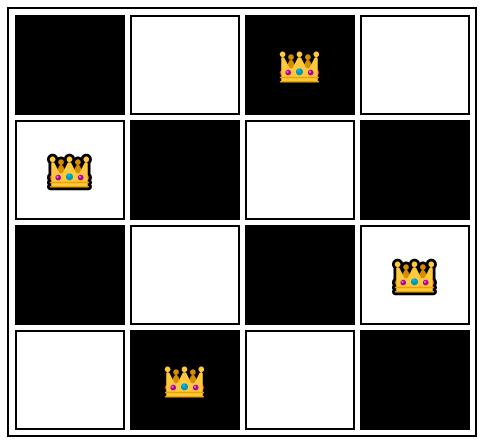
\includegraphics{pictures/4-Queens-Output.PNG}
    \caption{The rendered output for the $4$-Queens Problem. }
    \label{fig:n-Queens-Grafik}
\end{figure}



\appendix

\section{The \DiMo Tool}

\subsection{License}
As of version 0.2.1, \DiMo is available via GitHub under the BSD-3-Clauses licence.


\subsection{Installation}

The \DiMo testing tool is written in OCaml using version 4.08.0. The simplest way to use the tool is to install the OCaml package manager 
\texttt{Opam}\footnote{\url{https://opam.ocaml.org/}}. Make sure you use version 2 of \texttt{Opam}. For correct functionality, version 0.7.1 of the Opam package 
\texttt{ocaml-sat-solvers}\footnote{\url{https://opam.ocaml.org/packages/ocaml-sat-solvers/ocaml-sat-solvers.0.7.1}} is needed which is not installed with previous versions of Opam.

Opam then gives a simple way to install the OCaml compiler and runtime environment. To use the precompiled byte code version this should suffice. To compile a native 
version of the \DiMo tool one needs additional components that can be installed via \texttt{Opam}. See the file \texttt{README} for details.

\section{Syntax of the \DiMo Language}

The syntax of the \DiMo input language is given by the following grammar.
\begin{align*}
\nonterm{Main} ::=\ & \nonterm{Problem} \optional{\term{PROPOSITIONS} \nonterm{Props}}\ 
                                         \optional{\term{PARAMETERS} \nonterm{Params}}\ 
                                         \optional{\term{FORMULAS} \nonterm{Defs}}  \nonterm{OutLang}\\
\nonterm{Problem}\ ::=\ & \term{SATISFIABLE} \nonterm{Formula} \\
                 \altn & \term{VALID} \nonterm{Formula} \\
                 \altn & \term{EQUIVALENT} \nonterm{Formula} \term{TO} \nonterm{Formula} \\
                 \altn & \term{MODELS} \nonterm{Formula} \\
\nonterm{Props} ::=\ & \epsilon \altn \nonterm{Ident} \Big(\term{,} \nonterm{Ident}\Big)^* \\
\nonterm{Ident} ::=\ & \enumset{\texttt{A},\ldots,\texttt{Z}}\enumset{\texttt{A},\ldots,\texttt{Z},\texttt{a}\ldots,\texttt{z},\texttt{0},\ldots,\texttt{9},\term{\_}}^*\enumset{\term{'}}^* \\
\nonterm{Params} ::=\ & \nonterm{Var} \term{:} \nonterm{Domain} \Big( \term{,} \nonterm{Var} \term{:} \nonterm{Domain} \Big)^* 
                           \optional{\term{WITH} \nonterm{Constr}} \\
\nonterm{Var} ::=\ & \enumset{\texttt{a},\ldots,\texttt{z}}\enumset{\texttt{A},\ldots,\texttt{Z},\texttt{a}\ldots,\texttt{z},\texttt{0},\ldots,\texttt{9},\term{\_}}^*\enumset{\term{'}}^* \\ 
\nonterm{Domain} ::=\ & \term{Nat} \\
                \altn & \term{\{} \nonterm{Number} \term{,} \optional{\nonterm{Number} \term{,}} \term{..} 
                                         \optional{\term{,} \nonterm{Number}} \term{\}} \\
                \altn & \term{\{} \nonterm{Number} \group{\term{,} \nonterm{Number}}^* \term{\}} \\
\nonterm{Number} ::=\ & \enumset{\texttt{1},\ldots,\texttt{9}}\enumset{\texttt{0},\ldots,\texttt{9}}^* \\ 
\nonterm{Constr} ::=\ & \nonterm{Var} \nonterm{Cmp} \nonterm{Var} \group{\term{,} \nonterm{Var} \nonterm{Cmp} \nonterm{Var}}^* \\
\nonterm{Cmp} ::=\ & \term{=} \altn \term{<=} \altn \term{>=} \altn \term{<} \altn \term{>} \altn \term{<>} \\ 
\nonterm{Defs} ::=\ & \epsilon \altn \nonterm{Pattern} \term{=} \nonterm{Formula} \group{\term{,} \nonterm{Pattern} \term{=} \nonterm{Formula}}^* \\
\nonterm{Pattern} ::=\ &\nonterm{Ident} \optional{\term{(} \nonterm{Atom} \group{\term{,} \nonterm{Atom}}^* \term{)}} \\
\nonterm{Atom} ::=\ &\nonterm{Var} \altn \nonterm{Number} \\
\nonterm{Formula} ::=\ & \term{True} \altn \term{False} \altn \nonterm{Pred} \\
                 \altn & \term{(} \nonterm{Formula} \term{)} \\
                 \altn & \term{-} \nonterm{Formula} \altn \nonterm{Formula} \nonterm{Junct} \nonterm{Formula} \\
                 \altn & \nonterm{GenJunct} \nonterm{Var} \term{:} \nonterm{FinSet} \term{.} \nonterm{Formula} \\
\nonterm{Junct} ::=\ & \term{\&} \altn \term{|} \altn \term{->} \altn \term{<->} \\
\nonterm{GenJunct} ::=\ & \term{FORALL} \altn \term{FORSOME} \\
\nonterm{Pred} ::=\ & \nonterm{Ident} \optional{\term{(} \nonterm{Term} \group{\term{,} \nonterm{Term}}^* \term{)}} \\
\nonterm{Term} ::=\ & \nonterm{Atom} \altn \term{(} \nonterm{Term} \term{)} \altn \nonterm{UnOp} \nonterm{Term} \altn \nonterm{Term} \nonterm{BinOp} \nonterm{Term} \altn \nonterm{AccOp} \nonterm{FinSet} \\
\nonterm{UnOp} ::=\ & \term{LOG} \altn \term{FLOG} \\
\nonterm{BinOp} ::=\ &\term{+} \altn \term{-} \altn \term{*} \altn \term{\textasciicircum} \altn \term{MOD} \\
\nonterm{AccOp} ::=\ &\term{MIN} \altn \term{MAX} \\
\nonterm{FinSet} ::=\ & \term{\{} \nonterm{Term} \term{,} \optional{\nonterm{Term} \term{,}} \term{..} \term{,} \nonterm{Term} \term{\}} \\
                \altn & \term{\{} \nonterm{Term} \group{\term{,} \nonterm{Term}}^* \term{\}} \\
                \altn & \nonterm{FinSet} \nonterm{SetOp} \nonterm{FinSet} \\
\nonterm{SetOp} ::=\ & \term{\&} \altn \term{|} \altn{-} \\
\nonterm{OutLang} ::=\ & \term{OUTPUT} \nonterm{OutProg} \\
\nonterm{OutProg} ::=\ & \term{SKIP} 
          \altn \term{EXIT}
          \altn \term{PRINT} \nonterm{String}
          \altn \term{PRINTF} \nonterm{String} \term{(}\nonterm{Terms}\term{)}\\
          \altn & \term{IF} \nonterm{BExpr} \term{THEN} \nonterm{OutProg} \term{ELSE} \nonterm{OutProg} \term{UNDEF} \nonterm{OutProg} \term{ENDIF}\\
          \altn & \term{FOR} \nonterm{Ident} \term{OF OF PROPOSITIONS DO} \nonterm{OutProg} \term{DONE}\\
          \altn & \term{FOR} \nonterm{Var} \term{FROM} \nonterm{Term} \term{TO} \nonterm{Term} \term{STEP} \nonterm{Term} \term{DO} \nonterm{OutProg} \term{DONE}\\
          \altn & \nonterm{OutProg} \nonterm{OutProg}\\
 \nonterm{BExpr} ::=\ & \term{HASMODEL} \altn \nonterm{Props}\term{(} \nonterm{Term} \optional{ \group{\term{,} \nonterm{Term}}^* } \term{)}\altn \nonterm{Term} \nonterm{cmp} \nonterm{Term}\\
    \altn & \nonterm{BExpr} \& \nonterm{BExpr} \altn \nonterm{BExpr} | \nonterm{BExpr} \altn \neg \nonterm{BExpr} \\
\nonterm{String} ::=\ & \term{"} \group{\Sigma \setminus \term{"}}^* \term{"}
\end{align*}
A note to the \term{PRINTF} command: here use the \DiMo tool the normal printf syntax from conventional programming languages, where each substring \%i is replaced by the corresponding \nonterm{term} value.\\
\ \\
A note regarding precedences: the \DiMo tool implements the standard precedence rules for Boolean operators, i.e.\ \texttt{A \& B | C} is parsed in the same way as
\texttt{(A \& B) | C}. 

The precedence and associativity rules for the arithmetic operators are as follows: Addition, subtraction, multiplication and division are left-associative; exponentiation is 
right-associative. This enumeration also reflects the increasing order of precedence amongst these operations.


\section{Version History}

%Bug fixes:
%\begin{itemize}
%\item 
%\end{itemize}
\subsubsection*{Version 0.3.0 (25/11/2022)}
Feature changes:
\begin{itemize}
\item Add output control
\item Change to ocam-sat-solvers version 0.7.1
\end{itemize}

\subsubsection*{Version 0.2.3 (21/06/2021)}

Bug fixes:
\begin{itemize}
\item Fixed throwing of \texttt{exception Invalid_argument("Bytes.create")} on instances with long (or many) parameter names.
\end{itemize}

\subsubsection*{Version 0.2.2 (01/07/2020)}

Feature changes:
\begin{itemize}
\item Output of Boolean constants has been changed to match input, now \texttt{True} and \texttt{False}
\item The format of variables and formulas has been extended to allow quote symbols in the end as in \texttt{x'} etc.
\end{itemize}

\subsubsection*{Version 0.2.1 (29/10/2019)}

Feature changes:
\begin{itemize}
\item \DiMo has moved to GitHub under the BSD-3-Clauses license.
\end{itemize}


\subsubsection*{Version 0.2.0 (10/09/2019)}

Bug fixes:
\begin{itemize}
\item The tokenizer did not recognise line breaks properly so that failure because of lexing errors resulted in error messages reporting the line and column number wrongly. Fixed.
\item Applying the LOG function to argument 0 does not result in a stack overflow anymore. Instead the program terminates with failure. 
\end{itemize}
Feature changes:
\begin{itemize}
\item The \DiMo language has been extended with a function FLOG on terms that computes the rounded-off logarithm to base 2.
\item The standard precedence and associativity rules for the arithmetic operators have been implemented. The \DiMo language has been extended with a function FLOG on terms that computes the rounded-off logarithm to base 2.
\end{itemize}


\subsubsection*{Version 0.1.5 (03/07/2019)}

Bug fixes:
\begin{itemize}
\item Operator MAX was interpreted as MIN: fixed.
\end{itemize}


\subsubsection*{Version 0.1.4 (01/07/2019)}

Bug fixes:
\begin{itemize}
\item Command line parameters \texttt{--onlypos} and \texttt{--onlyneg} no longer ignored in checking validity problems.
\item Problem with non-atomic terms like \texttt{i+1} in set definitions, leading to program crashes with error ``\texttt{compare: invalid argument}'', fixed.
\item Problem with instantiation of formula schemes into negation normal form fixed.
\end{itemize}
Feature changes:
\begin{itemize}
\item Model enumeration problems now report the number of models that were found.
\end{itemize}

\subsubsection*{Version 0.1.2 (27/11/2018)}
Bug fixes:
\begin{itemize}
\item Faulty instantiation of formulas containing negation, generalised junctions (\texttt{FORALL}, \texttt{FORSOME}) and propositional constants (\texttt{True}, \texttt{False}) fixed.
\item Crash through array-out-of-bounds exception when specifying finite domains by enumeration of alle elements (e.g.\ \texttt{n:~\{1,2\}}) fixed.
\end{itemize}
Feature changes:
\begin{itemize}
\item Output in debug mode streamlined.
\item Added command-line parameters to suppress the printing of negative, resp.\ positive literals in models.
\end{itemize}

\subsubsection*{Version 0.1.1 (26/11/2018)}

Bug fixes:
\begin{itemize}
\item Problem with producing output for validity problems trying to show refuting assignments for valid rather than invalid formulas fixed. 
\item Program crashes due to an error in function ``toCNF.negate'' caused by non-literal arguments fixed. 
\end{itemize}

 
\bibliographystyle{plain}
\bibliography{../literature} 
\end{document}

